\documentclass[12pt,twoside]{report}

%%%%%%%%%%%%%%%%%%%%%%%%%%%%%%%%%%%%%%%%%%%%%%%%%%%%%%%%%%%%%%%%%%%%%%%%%%%%%

% Definitions for the title page
% Edit these to provide the correct information
% e.g. \newcommand{\reportauthor}{Timothy Kimber}

\newcommand{\reporttitle}{Title}
\newcommand{\reportauthor}{Your name}
\newcommand{\supervisor}{Name of supervisor}
\newcommand{\degreetype}{Type of Degree}

%%%%%%%%%%%%%%%%%%%%%%%%%%%%%%%%%%%%%%%%%%%%%%%%%%%%%%%%%%%%%%%%%%%%%%%%%%%%%

% load some definitions and default packages
%%%%%%%%%%%%%%%%%%%%%%%%%%%%%%%%%%%%%%%%%
% University Assignment Title Page 
% LaTeX Template
% Version 1.0 (27/12/12)
%
% This template has been downloaded from:
% http://www.LaTeXTemplates.com
%
% Original author:
% WikiBooks (http://en.wikibooks.org/wiki/LaTeX/Title_Creation)
%
% License:
% CC BY-NC-SA 3.0 (http://creativecommons.org/licenses/by-nc-sa/3.0/)
% 
%
%%%%%%%%%%%%%%%%%%%%%%%%%%%%%%%%%%%%%%%%%
%----------------------------------------------------------------------------------------
%	PACKAGES AND OTHER DOCUMENT CONFIGURATIONS
%----------------------------------------------------------------------------------------
\usepackage[a4paper,hmargin=2.8cm,vmargin=2.0cm,includeheadfoot]{geometry}
\usepackage{textpos}
\usepackage[nottoc]{tocbibind} % for bibliography
\usepackage{tabularx,longtable,multirow,subfigure,caption}%hangcaption
\usepackage{fncylab} %formatting of labels
\usepackage{fancyhdr} % page layout
\usepackage{url} % URLs
\usepackage[english]{babel}
\usepackage{amsmath}
\usepackage{graphicx}
\usepackage{dsfont}
\usepackage{epstopdf} % automatically replace .eps with .pdf in graphics
\usepackage{backref} % needed for citations
\usepackage{array}
\usepackage{latexsym}
\usepackage[pdftex,pagebackref,hypertexnames=false,colorlinks]{hyperref} % provide links in pdf
\usepackage{parskip}
\usepackage{float}
\usepackage{makecell}
\usepackage{xcolor}

% code type
\definecolor{light-gray}{gray}{0.95}
\newcommand{\code}[1]{\colorbox{light-gray}{\texttt{#1}}}

\hypersetup{pdftitle={},
  pdfsubject={}, 
  pdfauthor={},
  pdfkeywords={}, 
  pdfstartview=FitH,
  pdfpagemode={UseOutlines},% None, FullScreen, UseOutlines
  bookmarksnumbered=true, bookmarksopen=true, colorlinks,
    citecolor=black,%
    filecolor=black,%
    linkcolor=black,%
    urlcolor=black}

\usepackage[all]{hypcap}


%\usepackage{color}
%\usepackage[tight,ugly]{units}
%\usepackage{float}
%\usepackage{tcolorbox}
%\usepackage[colorinlistoftodos]{todonotes}
% \usepackage{ntheorem}
% \theoremstyle{break}
% \newtheorem{lemma}{Lemma}
% \newtheorem{theorem}{Theorem}
% \newtheorem{remark}{Remark}
% \newtheorem{definition}{Definition}
% \newtheorem{proof}{Proof}


%%% Default fonts
\renewcommand*{\rmdefault}{bch}
\renewcommand*{\ttdefault}{cmtt}



%%% Default settings (page layout)
\setlength{\parindent}{0em}  % indentation of paragraph

\setlength{\headheight}{14.5pt}
\pagestyle{fancy}
\renewcommand{\chaptermark}[1]{\markboth{\chaptername\ \thechapter.\ #1}{}} 

\fancyfoot[ER,OL]{\sffamily\textbf{\thepage}}%Page no. in the left on odd pages and on right on even pages
\fancyfoot[OC,EC]{\sffamily }
\renewcommand{\headrulewidth}{0.1pt}
\renewcommand{\footrulewidth}{0.1pt}
\captionsetup{margin=10pt,font=small,labelfont=bf}


%--- chapter heading

\def\@makechapterhead#1{%
  \vspace*{10\p@}%
  {\parindent \z@ \raggedright \sffamily
    \interlinepenalty\@M
    \Huge\bfseries \thechapter \space\space #1\par\nobreak
    \vskip 30\p@
  }}

%---chapter heading for \chapter*  
\def\@makeschapterhead#1{%
  \vspace*{10\p@}%
  {\parindent \z@ \raggedright
    \sffamily
    \interlinepenalty\@M
    \Huge \bfseries  #1\par\nobreak
    \vskip 30\p@
  }}

\allowdisplaybreaks

% load some macros
% Here, you can define your own macros. Some examples are given below.

\newcommand{\R}[0]{\mathds{R}} % real numbers
\newcommand{\Z}[0]{\mathds{Z}} % integers
\newcommand{\N}[0]{\mathds{N}} % natural numbers
\newcommand{\C}[0]{\mathds{C}} % complex numbers
\renewcommand{\vec}[1]{{\boldsymbol{{#1}}}} % vector
\newcommand{\mat}[1]{{\boldsymbol{{#1}}}} % matrix


\date{\today}

\begin{document}

% load title page
% Last modification: 2015-08-17 (Marc Deisenroth)
\begin{titlepage}

\newcommand{\HRule}{\rule{\linewidth}{0.5mm}} % Defines a new command for the horizontal lines, change thickness here


%----------------------------------------------------------------------------------------
%	LOGO SECTION
%----------------------------------------------------------------------------------------


\includegraphics[width = 4cm]{./figures/imperial}\\[0.5cm] 

\center % Center remainder of the page

%----------------------------------------------------------------------------------------
%	HEADING SECTIONS
%----------------------------------------------------------------------------------------

\textsc{\Large Imperial College London}\\[0.5cm] 
\textsc{\large Department of Computing}\\[0.5cm] 

%----------------------------------------------------------------------------------------
%	TITLE SECTION
%----------------------------------------------------------------------------------------

\HRule \\[0.4cm]
{ \huge \bfseries \reporttitle}\\ % Title of your document
\HRule \\[1.5cm]
 
%----------------------------------------------------------------------------------------
%	AUTHOR SECTION
%----------------------------------------------------------------------------------------

\begin{minipage}{0.4\textwidth}
\begin{flushleft} \large
\emph{Author:}\\
\reportauthor % Your name
\end{flushleft}
\end{minipage}
~
\begin{minipage}{0.4\textwidth}
\begin{flushright} \large
\emph{Supervisor:} \\
\supervisor % Supervisor's Name
\end{flushright}
\end{minipage}\\[4cm]


%----------------------------------------------------------------------------------------
%	FOOTER & DATE SECTION
%----------------------------------------------------------------------------------------
\vfill % Fill the rest of the page with whitespace
Submitted in partial fulfillment of the requirements for the MSc degree in
\degreetype~of Imperial College London\\[0.5cm]

\makeatletter
\@date 
\makeatother


\end{titlepage}



% page numbering etc.
\pagenumbering{roman}
\clearpage{\pagestyle{empty}\cleardoublepage}
\setcounter{page}{1}
\pagestyle{fancy}

%%%%%%%%%%%%%%%%%%%%%%%%%%%%%%%%%%%%
\begin{abstract}
Your abstract.
\end{abstract}

\cleardoublepage
%%%%%%%%%%%%%%%%%%%%%%%%%%%%%%%%%%%%
\section*{Acknowledgments}
Comment this out if not needed.

\clearpage{\pagestyle{empty}\cleardoublepage}

%%%%%%%%%%%%%%%%%%%%%%%%%%%%%%%%%%%%
%--- table of contents
\fancyhead[RE,LO]{\sffamily {Table of Contents}}
\tableofcontents 


\clearpage{\pagestyle{empty}\cleardoublepage}
\pagenumbering{arabic}
\setcounter{page}{1}
\fancyhead[LE,RO]{\slshape \rightmark}
\fancyhead[LO,RE]{\slshape \leftmark}

%%%%%%%%%%%%%%%%%%%%%%%%%%%%%%%%%%%%
\chapter{Introduction}
\label{Introduction}

%\begin{figure}[tb]
%\centering
%
\includegraphics[width = 0.4\hsize]{./figures/imperial}
%%\caption{Imperial College Logo. It's nice blue, and the font is quite stylish. But you can choose a different one if you don't like it.}
%\label{fig:logo}
%\end{figure}

%Figure~\ref{fig:logo} is an example of a figure. 
\begin{figure}
    \centering
    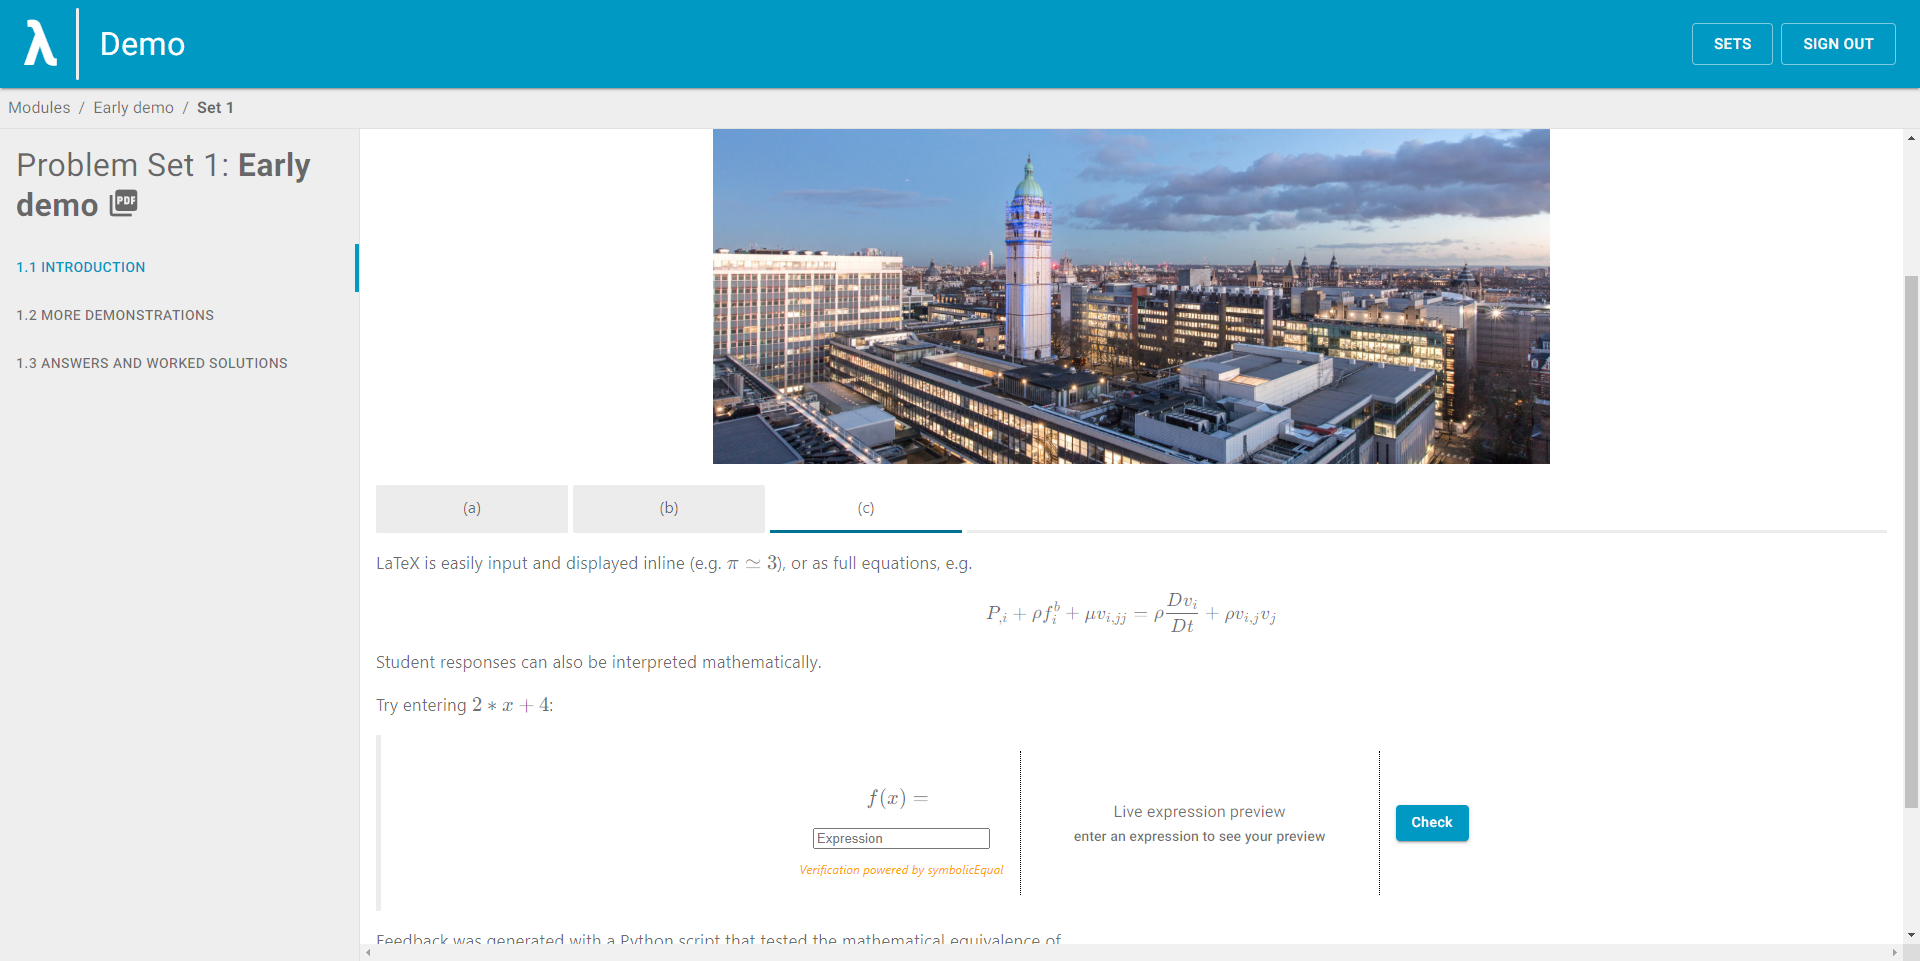
\includegraphics[width=\hsize]{figures/lambdafeedback-screenshot.png}
    \caption{Screenshot of a Demo in Lambada Feedback System}
    \label{fig:demoscreenshot}
\end{figure}

The application of remote learning in higher education has increased massively
since the explosion of COVID-19 \cite{remotelearning}. Many institutions including Imperial College
London moved their courses online during lockdowns. These courses are taught
based on online systems. However, some online systems are not capable of
conducting the digitalisation of teaching tasks such as lecture
recording/playing and assignment marking etc. For example, some departments of  Imperial College
London were using Möbius for online assignment and assessment, but it was complained by students and staffs that the system was hard to use. This thus leads to a demand of updating or developing new systems so that students and teachers can get better experience.

Therefore, the college has decided to develop a new online learning system named
Lambda Feedback. This system is a web application which allows students to do assignments posted by teachers and get feedback immediately. Comparing to its predecessor Möbius, Lambda
Feedback has modern user interface, friendly interaction and much more features.
One of the features is the expression input. In many assignment questions,
solutions are math expressions. In Lambda Feedback, users can input math
expressions in a text field, and the system is able to understand the expression
and check if it is correct. Figure \ref{fig:demoscreenshot} is a screenshot of a
demo in Lambda Feedback. The webpage displays a navigation sidebar,
the question, and the answer area, where users can input the expression.

However, the current system only supports keyboard input for math expressions.
Users need to type the whole expression including symbols and operators, which
can be very inconvenient and complex especially for complicated equations.
Consequently, an extension with a new method of input is needed for the system.

Handwriting input is considered appropriate for the system because of its
convenience and simplicity. Although there are other input methods such as
equation editor and image upload, they either require users to learn how to use,
or need some extra steps. This means they are not suitable as the major approach
of expression input, but can be a good supplement to handwriting input in some
special situations.

This project thus aims to develop a component with handwriting input and
equation recognition, and integrate it to the Lambda Feedback system. The
component shall enable the users to write on it either via mouse/touchpad on
computers or fingers/pens on mobile devices. After users finish input, it should
be able to recognize the equation and display the result alongside the writing
area. Integration with the Lambda Feedback system should be carried out after
the component is tested available.

This report records the development of the project. Chapter \ref{Background}
investigates several approaches to realise the software component and analyses
their advantages and drawbacks. Chapter \ref{Implementation} states the progress
of development and explains the implementation of the software component. In
Chapter \ref{Results}, progressive results are demonstrated and the final
achievement is shown. An evaluation of the results are included in this chapter
as well. Finally, in chapter \ref{Conclusion}, a conclusion of the project is drawn, and possible future improvements are listed.



%%%%%%%%%%%%%%%%%%%%%%%%%%%%%%%%%%%%
\chapter{Background}
\label{Background}

This chapter records the background research, which includes general reviews on
articles, tutorials and existing projects that have helped the development of
this project, as well as potential choices that could be taken and why they were
discarded, along with the reasons of selecting current tools. An overview of the project is made below before diving into details.

\section*{Overview}
\label{bgOverview}

The component to develop is a TypeScript (strong typed version of JavaScript) web application which has two major functionalities:
\begin{enumerate}
    \item Have a canvas where users can write equation
    \item Ability to recognise the equation written on canvas and display the result
\end{enumerate}

Moreover, the component should be integrated into Lambda Feedback, so it is necessary to introduce the system because they will use same frameworks and language.

Lambda Feedback is a web application which has a frontend and a backend.
The frontend is built upon \textit{NextJS} (a framework built on \textit{React}), and the backend is built upon \textit{NestJS}. Both
are written in Typescript (These frameworks will be introduced in Chapter \ref{bgIntegrationLF}). The major part of the project will be installed in a component of the frontend named \textit{ResponseArea}, which is responsible for receiving input and giving result to users.

It is difficult to develop the component directly upon Lambda Feedback, as it
already had much code when this project launched. Therefore, it was decided to
build a web application independent of Lambda Feedback to save time on reading
code and testing functionality.

Although the final independent web application must be written under the same
framework with Lambda Feedback, i.e. \textit{React}, there is another way,
\textit{Vanilla JavaScript} (also referred to as plain JS), to start with. Table \ref{MethodComparison} compares the two methods:
\begin{table}[H]
    \centering
    \caption{Comparison of Two Methods for Independent Web Application}
    \label{MethodComparison}
    \begin{tabular}{|m{0.15\textwidth}|m{0.4\textwidth}|m{0.3\textwidth}|}
        \hline
        \textbf{Method} & \textbf{Advantages} & \textbf{Disadvantages}\\
        \hline
        Vanilla JavaScript & Easy to start \& Require no extra configuration&
        Does not fit Lambda Feedback\\
        \hline
        React & Uses same framework as Lambda Feedback - does not need extra steps for integration & Need to study React before start\\
        \hline
    \end{tabular}
\end{table}
After careful consideration, it was decided to start by using \textit{Vanilla JavaScript} to get familiar with functionalities, and then converting the application to \textit{React}. This makes the procedure more fluent and only need to focus on one emphasis for every progress.

Overall, the procedure of the project is:
\begin{enumerate}
    \item Develop a web application with \textit{Vanilla JavaScript} which enables users to draw equations, and recognise the equation
    \item Move the web application under \textit{React} framework
    \item Integrate the application as a component to Lambda Feedback
\end{enumerate}


Despite using different frameworks during the procedure, the approaches to realise functionalities are the same. Hence, the background research mainly focuses on three parts:
\begin{itemize}
    \item A canvas where users can draw stuffs
    \item Functionality of mathematical equation recognition
    \item \textit{React} framework and integration with the Lambda Feedback
\end{itemize}
Therefore, the remaining part of this chapter is divided into three sections, each introducing one part. 

\section{Canvas}
\label{bgCanvas}
A handwriting canvas is needed for the component, which should do the following:
\begin{itemize}
    \item Users can draw and edit stuffs
    \item The canvas can output the content, either by image or stroke data
\end{itemize}
Here, stroke data means positions that represent points on the strokes. For
example, stroke \code{\{1, 1\}, \{2, 2\}, \{3, 3\}} means a line starting at point (1, 1), passing point (2, 2) and ends at (3, 3). All paths drawn on the canvas can be expressed as stroke data.

Two HTML elements - \code{canvas} and \code{SVG} - were investigated for this part.

The \code{canvas} element is an HTML container used
to draw graphics on web page. Graphics are drawn by APIs, which has several
methods for drawing, including paths, boxes, circles, text, and adding images
\cite{webcanvas}. 

The component can utilize its paths method to display the user's strokes: once the user drags the pointer, the component fetches its position in the canvas, and draws a path to the next position the pointer moves to. 

The \code{canvas} element also provides APIs to output content as images, while stroke data is generated when recording positions of the pointer.

Drawing on \code{canvas} is easy because all graphics is drawn by APIs, so the component only needs to 'tell' \code{canvas} how to draw. However, there are two drawbacks of this element: 
\begin{enumerate}
    \item To use \code{canvas} APIs, the HTML element should be referred. This in \textit{React} will be using \code{React Refs}. Unlike in \textit{Vanilla JS}, API callings in \textit{React} should be carefully considered with \textit{React Component Lifecycle} \cite{webreactlife}. This will affect the performance of the component and brings extra work.
    \item The \code{canvas} element is represented as a Bitmap in webpage. This means when transforming the size of the canvas, graphics might look blurry \cite{webcanvasvssvg}. This will be further discussed in Chapter \ref{Implementation}.
\end{enumerate}

In contrast with \code{canvas}, the \code{SVG} element does not have listed
problems. The term SVG (Scalable Vector Graphics) means an XML based vector
image format for defining 2D graphics. Therefore, as an element in HTML,
\code{SVG} simply represents a container for SVG graphics.

Because it is 'vector graphic', regardless of the ratio of rendered size and
programmed size, users can always get a clear graph of what they draw. This thus
solve the blurry problem of \code{canvas}.

\code{SVG} has several sub-element including \code{Path}. Data of a \code{Path} is a string containing commands and points, and is attached to its property 'd'. 

To show strokes that a user draws, instead of containing them in one \code{canvas} element, multiple \code{Path}s are used to display the user's drawing, each for one stroke. It is more flexible for the programme to monitor and control them. 

This feature fits \textit{React Component Lifecycle} perfectly as any change of path data causes \textit{React} to 'react' to it, and render the path with updated data.

Overall, \code{SVG} is more suitable than \code{canvas} for this project due to its vector property and compatibility with \textit{React}.



\section{Equation Recognition}
\label{bgEqnRecognition}




\section{Integration with Lambda Feedback}
\label{bgIntegrationLF}



%%%%%%%%%%%%%%%%%%%%%%%%%%%%%%%%%%%%
\chapter{Implementation}
\label{Implementation}


%%%%%%%%%%%%%%%%%%%%%%%%%%%%%%%%%%%%
\chapter{Experimental Results}
\label{Results}


%%%%%%%%%%%%%%%%%%%%%%%%%%%%%%%%%%%%
\chapter{Conclusion}
\label{Conclusion}


%% bibliography
\bibliographystyle{vancouver}
\bibliography{mybibs}

\end{document}
